
\chapter{An Empirical Application\label{chap:6}}

In this chapter, we apply the methods developed in this thesis to
model the evolution of conditional expectations of inflation among
professional economic forecasters.


\section{The Survey of Professional Forecasters}

We introduce the data we intend to explore and formalize the modeling
problem in this section. The European Central Bank (ECB), along with
other major central banks around the world, carries out a quarterly
survey of expectations for the rate of inflation among professional
economists and institutions, known as the Survey of Professional Forecasters
(SPF). We refer the reader to ECB publications such as \citet{ecb-review}
for a detailed review of the ECB's SPF. Though the format of the SPF
has evolved over time, in every SPF since the first quarter of 1999
(1999Q1), a panel of professional forecasters has been asked to provide
their expectations of annualized HICP Euro Area inflation at the end
of the current calendar year, the next calendar year, and the calendar
year five years ahead. Recent SPFs have also included forecasts for
the end of the calendar year after next. The ECB reports the expectations
of all surveyed forecasters at every horizon included in the SPF questionnaire,
indexing the forecasts by the forecaster who provided them. \figref{ecb_intuition}
visualizes SPFs from two contrasting macroeconomic regimes to give
an intuitive sense of the shape of the data.

\begin{figure}[H]
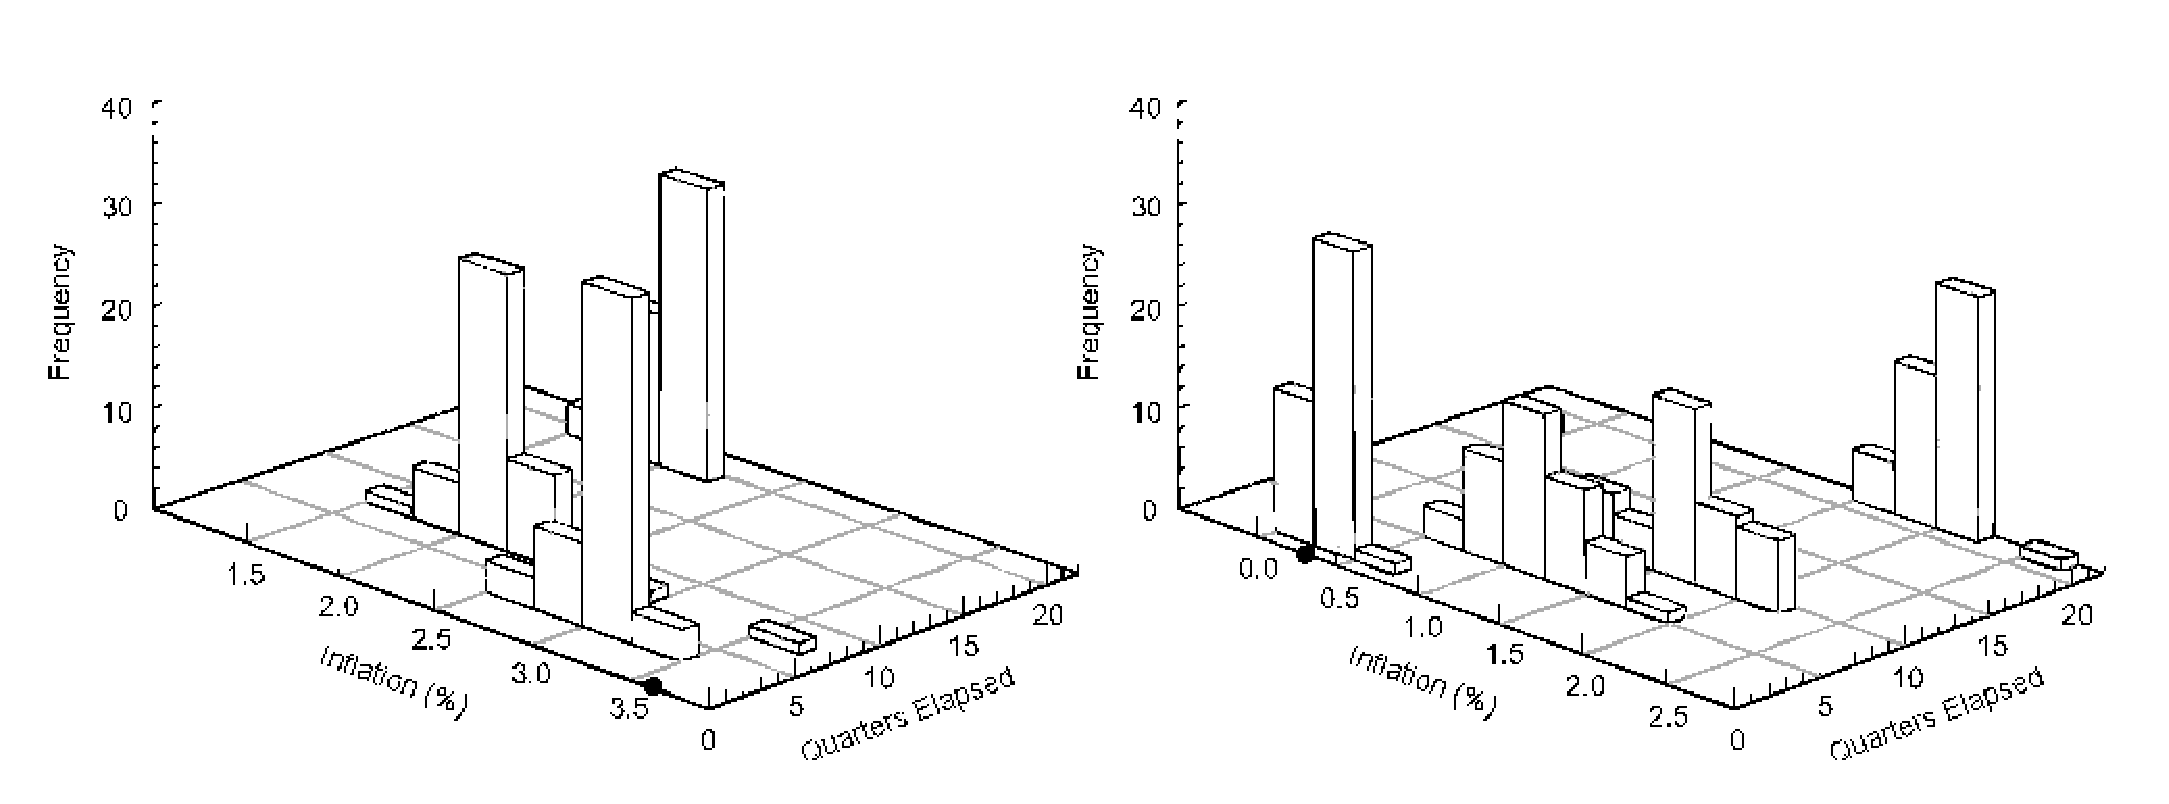
\includegraphics[width=1\columnwidth]{/Users/marshall/Documents/senior/thesis/figures/ecb_intuition_ed_tall_vector}

\caption{\label{fig:ecb_intuition}The marginal distribution of inflation forecasts
at the horizons included in the 2008Q2 (left) and 2009Q4 (right) SPFs.
The black dot indicates the inflation rate as of the month before
the SPF was administered.}
\end{figure}


The prices of many financial securities (inflation-indexed bonds,
for instance; see \citet[Eq. 2 in][]{woodward-1990}) depend on inflation
expectations over time. Given the vast array of inflation-linked securities
in the marketplace, the forecast horizons of the SPF may be too coarse
to be useful for practical purposes: for instance, we may be interested
in the distribution of inflation expectations halfway through a calendar
year. Thus emerges a natural arena in which we may ask questions of
inference and imputation given distributional data.

We formalize the problem as follows. Suppose we have an uncountable
sample space $\Omega$ of forecasters, each with her own model for
the evolution of HICP Euro Area inflation over time given current
inflation. We define the inflation expectation process $X=\{X_{t}\}$
where $X_{t}(\omega)$ is $\Omega\ni\omega$'s conditional expectation
for inflation at time horizon $t$ given current inflation. Furthermore,
we suppose $X$ evolves according to some model $\mathbb{P}$ that
is entirely unknown to us (the only constraint for this section that
we place on $\mathbb{P}$ is that it is absolutely continuous with
respect to the Gaussian measure). With this setup, the data provided
in any particular SPF are discrete observations of some finite number
of sample paths of $X$ under $\mathbb{P}$.

We are interested in what a particular SPF can tell us about the underlying
dynamics of the evolution of inflation expectations, and how we can
impute the distribution of $X$ at horizons not included in the SPF
questionnaire. The latter question can be intuitively understood as
asking what the forecasters would have said if we had surveyed them
for their inflation expectations at an arbitrary horizon. In the following
section, we will work with the $M=68$ SPFs conducted by the ECB from
1999Q1 through 2015Q4, obtained at \citep{spf-site}. \tabref{summary}
provides some summary statistics of this dataset.

\begin{table}
\centering \begin{tabular}{@{}lllll@{}} \toprule                                     & Mean  & SD   & Min.  & Max. \\ \midrule Forecasters surveyed                & 103.5 & 7.6  & 94    & 116  \\ Forecasters with complete responses & 44.3  & 6.1  & 33    & 62   \\ Inflation at time of SPF (\%)       & 1.76  & 0.90 & -0.70 & 4.10 \\ SD of nearest horizon forecasts (\%)     & 0.15  & 0.05 & 0.05  & 0.33 \\ SD of farthest horizon forecasts (\%)    & 0.21  & 0.07 & 0.09  & 0.55 \\ \bottomrule \end{tabular}

\begin{centering}
\begin{tabular}{lllll>{\raggedright}m{2cm}}
\multirow{1}{*}{} & \multirow{1}{*}{} &  &  &  & \tabularnewline
\end{tabular}
\par\end{centering}

\caption{\label{tab:summary}Summary statistics for the $68$ ECB SPFs administered
from 1999Q1 through 2015Q4.}
\end{table}



\section{Simple Inference on Inflation Expectations}

In this brief section, we verify that the proposed MCEM algorithm
consistently estimates the MKLDE in an empirical setting. In particular,
we posit a probability model $\mathbb{Q}_{\theta}$ under which $X$
is an OU diffusion governed by $\theta=(\mu,\lambda,\sigma)$. This
is an economically sensible model, consistent with the mean reversion
implicit in ECB's inflation targeting policy of aiming for ``inflation
rates of below, but close to, 2\% in the medium term'' \citep{targeting}.
Moreover, this is a mathematically convenient specification since
the transition density of the OU diffusion is analytically tractable.
We consider a particular SPF questionnaire, and let $\mathcal{T}=\{t_{1},\dots,t_{n}\}$
where $t_{1}>0$ be the set of horizons measured in quarters included
in the SPF and $\mathcal{O}\subseteq\Omega$ be the set of forecasters
with complete responses. Then, the average log-likelihood of the data
under $\mathbb{Q}_{\theta}$ is
\[
\bar{\ell}(\theta)=\frac{1}{|\mathcal{O}|}\sum_{\omega\in\mathcal{O}}\sum_{i=1}^{n}\mathcal{N}(X_{t_{i}}(\omega);\mu+(X_{t_{i-1}}(\omega)-\mu)e^{-\lambda t},\sigma^{2}(1-e^{-2\lambda t})/2\lambda),
\]
where $\mathcal{N}(x;\mu,\sigma^{2})$ is the Gaussian density with
mean $\mu$ and variance $\sigma^{2}$ and $X_{t_{i}}(\omega)$ is
forecaster $\omega$'s expectation of inflation at horizon $t_{i}$.
We set $X_{t_{0}}$ to the annualized HICP Euro Area inflation reported
at the end of the most recent month before the quarter that the SPF
was distributed (the SPF is usually distributed in the first month
of each quarter, so we can assume forecasters are conditioning on
the inflation print of the previous month). 

\begin{table}[b]
 \centering \begin{tabular}{@{}cccccl@{}} \toprule                         & Mean of $\theta^*$ & Bias (MCEM Est.)  &  \multicolumn{3}{l}{Cov. of bias ($\times 10^{-2}$)} \\ \midrule $\mu$             & 1.94 & -0.02\:            & \:1.23\:            &                &                \\ $\lambda$         & 0.23 & \;0.06\:           & -0.51\:           & 1.10           &                \\ $\sigma$          & 0.17 & \;0.00\:           & -0.56\:           & 0.50           & 0.24           \\ \bottomrule \end{tabular}


\begin{centering}
\begin{tabular}{lllll>{\raggedright}m{2cm}}
\multirow{1}{*}{} & \multirow{1}{*}{} &  &  &  & \tabularnewline
\end{tabular}
\par\end{centering}

\caption{\label{tab:mle-vs-mcem}Mean of the $\theta^{*}=\arg\max\bar{\ell}(\theta)$,
as well as the bias of MKLDE estimates, obtained by approximate MCEM,
relative to $\theta^{*}$, over $68$ ECB SPFs.}
\end{table}


By the comments in \chapref{EM}, $\arg\max\bar{\ell}(\theta)$, which
can be easily found through numerical optimization procedures, is
the parameter that asymptotically minimizes the K-L divergence of
the law of $X_{\mathcal{T}}$ under $\mathbb{Q}_{\theta}$ from its
law under $\mathbb{P}$. \tabref{mle-vs-mcem} reports the mean $\arg\max\bar{\ell}(\theta)$
and bias of the MKLDEs obtained through MCEM on the SPFs in our dataset,
measuring time in quarterly units. We note that the MKLDEs for $\mu$
and $\sigma$ obtained by approximate MCEM are effectively indistinguishable
from those obtained via direct maximization of the analytic likelihood.
Moreover, the MKLDE for $\mu$ aligns closely with intuition: On average,
forecasters seem to expect the reversion of inflation to the medium-term
inflation target of the ECB (below, but close to, $2\%$).

On the other hand, the bias is non-trivially positive for the MKLDE
of $\lambda$, suggesting that the thin-tailedness of the approximate
bridges can in fact affect the quality of approximate MCEM estimates
in empirical situations. The computational cost of exact MCEM, however,
can still be high enough that the practitioner will need to weigh
the utility of slightly more accurate estimates against significantly
longer running times on a case-by-case basis.


\section{Putting It All Together}

In the final original section of this thesis, we synthesize the methods
developed here by answering the following question: What can we say,
given a finite number of sample paths of $X$ observed at discrete
time points, about the distribution of $X$ at arbitrary horizons,
when the parameters governing $X$ are unknown? In particular, we
propose a generalized bridge-based imputation scheme given distributional
data and a stochastic model known only up to its parameters. We show
such a scheme reduces mean out-of-sample estimated K-L divergence
of interpolations from the truth vis-�-vis a baseline linear interpolation
for the ECB SPF dataset, using models with tractable and intractable
log-likelihood. 

To begin, we consider a particular SPF containing forecasts from a
finite set of forecasters at every time $t\in\mathcal{T}=\{t_{1},\dots,t_{n}\}$
where $t_{1}>0$. Let $\hat{\nu}$ be the $(n+1)$-dimensional empirical
distribution induced by these forecasts and the fixed inflation print
at $t_{0}=0$, the month before the SPF was administered (noting that
the dependence structure of this distribution is given by the indexing
of forecasts at different horizons to particular forecasters). Recall
that the forecasts contained in the SPF can be understood as samples
from $X_{\mathcal{T}}$ under the true but unknown model $\mathbb{P}$,
and let $\mathbb{P}_{X_{\mathcal{T}}}$ be the law of $X_{\mathcal{T}}$
under $\mathbb{P}$. 

\begin{figure}
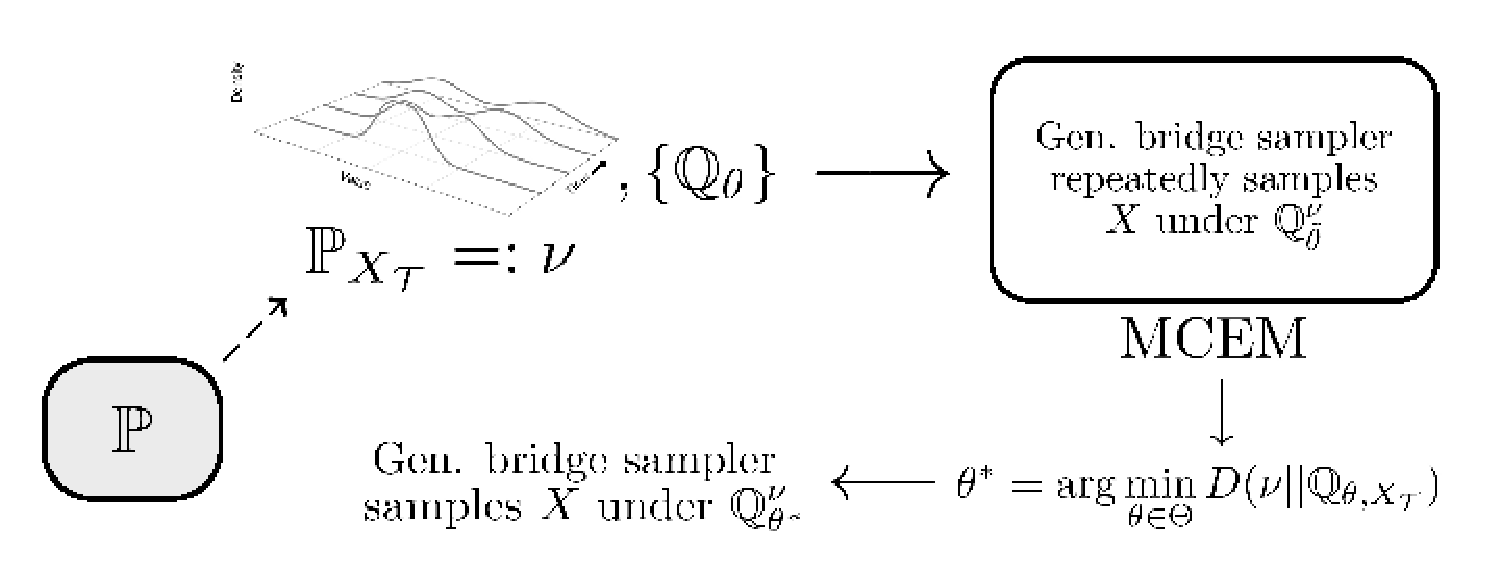
\includegraphics[width=1\columnwidth]{/Users/marshall/Documents/senior/thesis/figures/imputation_scheme}

\caption{\label{fig:imputation}A schematic depiction of the proposed imputation
method, in which the MCEM algorithm for estimating the MKLDE and the
generalized bridge samplers developed in previous chapters are used
to approximate the law of $X$ under $\mathbb{P}$ with samples from
$X$ under $\mathbb{Q}_{\theta^{*}}^{\nu}$. $\mathbb{P}$ is enclosed
in a grey box, highlighting that we do not have access to $\mathbb{P}$
but rather only the law of $X_{\mathcal{T}}$ under $\mathbb{P}$.}
\end{figure}


Now, fix a parameterized family of models $\{\mathbb{Q}_{\theta}\}$.
Suppose we have the parameter $\theta^{*}$ that minimizes the K-L
divergence of the distribution of $X_{\mathcal{T}}$ under $\mathbb{Q}_{\theta}$
from its true distribution $\mathbb{P}_{X_{\mathcal{T}}}$. We posit
that a reasonable guess for the law of $X$ under $\mathbb{P}$ when
only given $\mathbb{P}_{X_{\mathcal{T}}}$ is the law of $X$ under
the $(X_{\mathcal{T}},\mathbb{P}_{X_{\mathcal{T}}})$-conditioning
of $\mathbb{Q}_{\theta^{*}}$.\footnote{A theoretical justification of this statement is a pressing direction
for future research.} It follows that a natural imputation method for the distribution
of $X$ under $\mathbb{P}$ at arbitrary horizons, schematized in
\figref{imputation}, is to first estimate the MKLDE $\theta^{*}$,
then simulate $\mathbb{P}_{X_{\mathcal{T}}}$-bridges of $X$ under
$\mathbb{Q}_{\theta^{*}}$; here, we use $\hat{\nu}$ as a plug-in
estimate for $\mathbb{P}_{X_{\mathcal{T}}}$. \figref{imputation}
highlights how the questions of inference and imputation on distributional
data, and by extension the MCEM algorithm and the generalized bridge
samplers developed in \chapref{EM} and \chapref{4}, are intimately
related.

We cross-validate the proposed imputation method as follows, setting
\begin{aenumerate}
\item $\hat{\nu}_{t_{i}}$ to be the empirical distribution induced by the
forecasts at $t_{i}$,
\item $\hat{\nu}_{-t_{i}}$ to be the the $n$-dimensional empirical distribution
of the forecasts at all horizons except $t_{i}$, and
\item $X_{-t_{i}}\coloneqq X_{\mathcal{T}\setminus t_{i}}$.
\end{aenumerate}
\begin{figure}
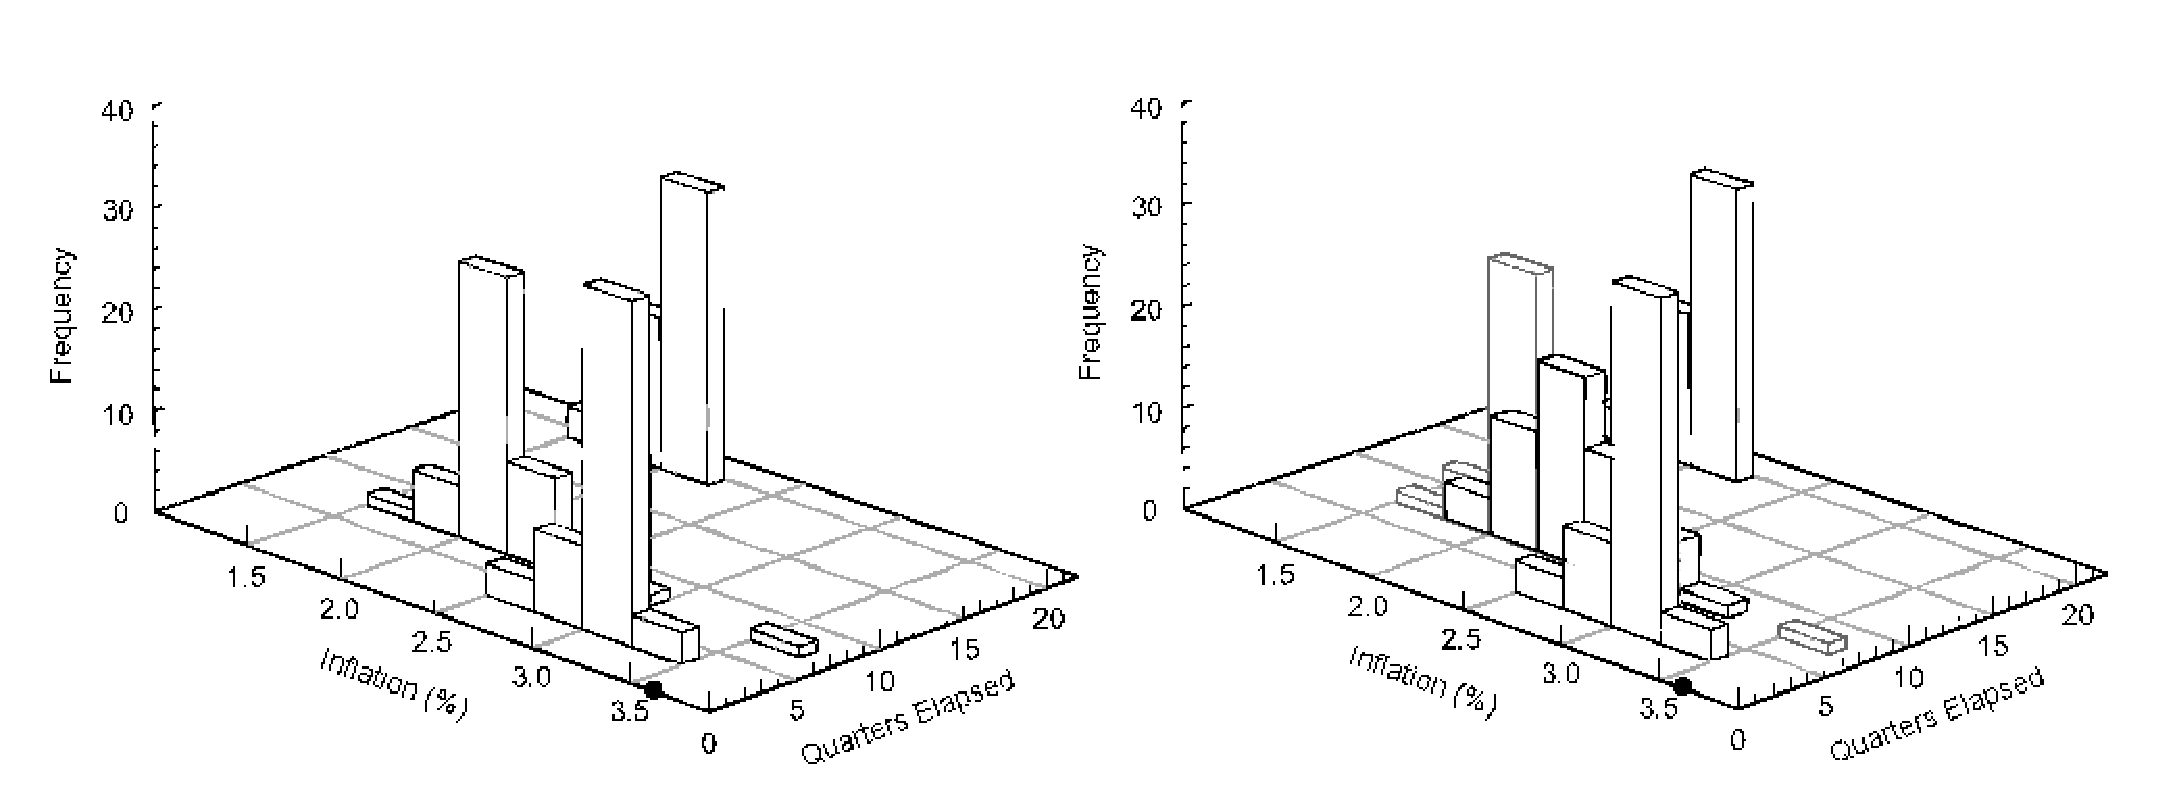
\includegraphics[width=1\columnwidth]{/Users/marshall/Documents/senior/thesis/figures/cross_v_intuition}

\caption{\label{fig:cv}A visualization of the cross-validation method for
assessing imputation strategy performance. The left graphic depicts
data from a particular SPF. The right graphic depicts an imputed distribution,
in black, superimposed on the original true distribution, to be used
to validate the imputated distribution, in gray.}
\end{figure}


First, we estimate the MKLDE $\theta_{-t_{i}}^{*}$ for $X$ under
$\mathbb{Q}_{\theta}$ given $\hat{\nu}_{-t_{i}}$ using approximate
MCEM. Then, we draw samples of $X_{t_{i}}$ under the Baudoin-$(X_{-t_{i}},\hat{\nu}_{-t_{i}})$
conditioning of $\mathbb{Q}_{\theta_{-t_{i}}^{*}}$ to induce an empirical
imputed distribution $\tilde{\nu}_{t_{i}}$. Finally, we use $\tilde{\nu}_{t_{i}}$
and $\hat{\nu}_{t_{i}}$ to consistently estimate the out-of-sample
Kullback-Liebler divergence of the law of $X_{t_{i}}$ under the Baudoin-$(X_{-t_{i}},\mathbb{P}_{X_{-t_{i}}})$
conditioning of $\mathbb{Q}_{\theta_{-t_{i}}^{*}}$ from its law under
$\mathbb{P}$ using the estimator of \citet[Theorem 1 in][]{perez-cruz-2008}.
Since forecasters often give the same forecasts for inflation at a
particular horizon, and the \citet{perez-cruz-2008} estimator requires
an empirical distribution function induced by unique samples, we add
arbitrarily small normally distributed noise $(\sigma^{2}\approx10^{-4})$
to the forecasts that induce $\hat{\nu}_{t_{i}}$. Furthermore, since
$n\geq3$ for all SPFs in our dataset, we consider $i\in\{1,2\}$.
\figref{cv} intuitively visualizes the cross-validation process:
The left side depicts the original SPF dataset, while the right side
depicts the removal of the marginal distribution at $t_{2}=8$ and
a new imputed marginal distribution at that time. The K-L divergence
of the imputed distribution from the grayed-out marginal distribution
is estimated as described.

To put the performance of our proposed imputation scheme into context,
we set a linear interpolation scheme as our baseline. In particular,
a linear interpolation $\tilde{X}_{t}$ of the forecasts $\{X_{t_{i}}\}_{t_{i}\in\mathcal{T}}$
of a particular forecaster is the function 
\begin{equation}
\tilde{X}_{t}=\frac{(t_{i}-t)X_{t_{i-1}}+(t-t_{i-1})X_{t_{i}}}{t_{i}-t_{i-1}}\label{eq:lininterp}
\end{equation}
for $t_{i-1}\leq t\leq t_{i}$ and $i=2,\dots,n$. This scheme is
not simply a straw man; its non-parametric nature makes it an extremely
robust imputation method, and it is simple to implement. Therefore,
in order for a complex scheme like the one proposed in this chapter
to be seen as a viable alternative for imputation, it must offer meaningful
improvements over linear interpolation. 

Our prior belief is that our scheme should in fact improve substantially
on linear interpolation. For instance, inflation expectations are
likely state-dependent: Central banks are wary of overshooting their
inflation targets, and thus can be expected to deploy monetary policy
to slow the velocity of inflation movements as inflation approaches
their target. A linear interpolation will not capture this expected
deceleration in inflation expectations while various It� diffusions,
including the OU diffusion, may be able to.

Though the case of an OU model was useful in the previous section
as an illustrative example, the development of an MCEM algorithm was
motivated by the fact that there are a wide range of diffusions for
which transition densities are not analytically available. As such,
in addition to a model $\mathbb{Q}_{\theta}^{OU}$ under which $X$
is an OU diffusion, we consider a model $\mathbb{Q}_{\theta}^{HYP}$
under which $X$ evolves according to 
\begin{equation}
dX_{t}=\frac{-\lambda(X_{t}-\mu)dt}{\sqrt{\delta^{2}+(X_{t}-\mu)^{2}}}+\sigma dW_{t},\label{eq:hypdiff}
\end{equation}
i.e. a model under which $X$ is a hyperbolic diffusion. This type
of diffusion was first proposed by \citet[Eq. 6.2 in][]{barndorff-1978},
who noted such a diffusion has stationary distribution 
\[
f(x)=\frac{e^{-\frac{2\lambda}{\sigma^{2}}\sqrt{\delta^{2}+(x-\mu)^{2}}}}{2\delta K_{1}(2\delta\lambda/\sigma^{2})},
\]
where $K_{1}$ is a modified Bessel function of the third kind with
index $1$. Hyperbolic diffusions are It� diffusions with finite speed
measure, and thus satisfy the assumptions made in \chapref{2}; however,
they do not admit a tractable transition density. We can see by inspection
of (\ref{eq:hypdiff}) that this model incorporates linear mean reverting
drift dynamics, similar to those of an OU process, when $|X_{t}-\mu|$
is small, and constant mean reverting drift when $|X_{t}-\mu|$ is
large. Since the hyperbolic diffusion, like the OU process, has constant
diffusion coefficient, its Lamperti transform and the requisite functions
for performing MCEM are easy to find.

\tabref{wilcoxon} presents the mean and median estimated K-L divergences
of the imputed distributions at $t_{1}$ and $t_{2}$ from the true
distributions over each SPF in the data set, using the generalized
bridge-based imputation scheme and the linear interpolation method
outlined in (\ref{eq:lininterp}). In all SPFs considered, $t_{1}$
and $t_{2}$ are time horizons between $1-4$ and $5-8$ quarters
respectively. 

\begin{table}[t]

\centering \begin{tabular}{@{}lccccm{0.1em}cc@{}} \toprule \multirow{2}{*}{Horizon \& Imputation Scheme} & \multirow{2}{*}{Mean} & \multirow{2}{*}{Median} & \multicolumn{2}{c}{Wilc. $p$ vs.}  & & \multicolumn{2}{c}{Sign $p$ vs.} \\ \cmidrule(l){4-5} \cmidrule(l){7-8}                                                             &         &                 & LI   & OU  & & LI   & OU                 \\ \midrule \emph{1-4 Quarter Horizon}                                  &         &                 &      &     & &      &                 \\ \:\:\:\:Linear Interpolation (LI)                           & 1.43    & 1.29            &      &     & &      &                    \\ \:\:\:\:Gen. Bridge (OU)                                    & 1.14    & 0.95            & 0.01 &     & & 0.08 &                    \\ \:\:\:\:Gen. Bridge (Hyp.)                                  & 1.18    & 0.96            & 0.00 & 0.61& & 0.14 & 0.85                  \\ \emph{5-8 Quarter Horizon}                                  &         &                 &      &     & &      &                 \\ \:\:\:\:Linear Interpolation (LI)                           & 0.96    & 0.81            &      &     & &      &                \\ \:\:\:\:Gen. Bridge (OU)                                    & 0.70    & 0.78            & 0.04 &     & & 0.23 &                  \\ \:\:\:\:Gen. Bridge (Hyp.)                                  & 0.74    & 0.61            & 0.01 & 0.15& & 0.09 & 0.32                \\
\bottomrule \end{tabular}


\begin{centering}
\begin{tabular}{lllll>{\raggedright}m{2cm}}
\multirow{1}{*}{} & \multirow{1}{*}{} &  &  &  & \tabularnewline
\end{tabular}
\par\end{centering}

\caption{\label{tab:wilcoxon}Mean and median out-of-sample estimated K-L divergences
of imputed inflation expectations from the distribution of $X$ under
$\mathbb{P}$ for various horizons and imputation schemes, across
$52$ SPFs (any SPFs for which approximate MCEM did not converge were
dropped). K-L divergences were estimated using the \citet{perez-cruz-2008}
estimator. If $X$ and $Y$ are the true K-L divergences under the
row and column imputation schemes, Wilcoxon $p$-values (Wilcox. $p$)
and sign $p$-values (Sign $p$) are obtained from the Wilcoxon signed-rank
test and the sign test respectively, under the alternative hypothesis
that $P(X-Y<0)>1/2$.}
\end{table}


\tabref{wilcoxon} also presents $p$-values from tests on the paired
differences of the K-L divergences between the various imputation
schemes; these can be used to evaluate the statistical significance
of the reductions in K-L divergence offered by a particular imputation
scheme over another. Exploratory data analysis suggests that the paired
differences of K-L divergences deviate substantially from normality;
\tabref{wilcoxon} therefore presents the $p$-values from a Wilcoxon
signed-rank test for whether the paired differences are centered at
zero. However, these paired differences also display some amount of
skew. Given the relatively small sample size ($52$ paired differences),
it is not clear whether this skewness suggests a material violation
of the symmetry assumption underlying the Wilcoxon signed-rank test;
as such, we also present $p$-values obtained from the sign test,
whose few assumptions can be confirmed to be satisfied by our data.

We see that the generalized bridge-based methods offer qualitatively
large reductions (on the order of $20-30\%$) in the mean and median
of out-of-sample estimated K-L divergences vis-�-vis a linear interpolation
scheme, at both horizons considered. The Wilcoxon signed-rank test
reveals that the improvements over the linear interpolation scheme
offered by our generalized bridge-based methods are statistically
significant at the $95\%$, and sometimes $99\%$, level. The sign
test, on the other hand, only begins to reveal significant differences
at the $90\%$ level; however, we ought to keep in mind that the sign
test is an extremely conservative test that discards any information
about the magnitude of the K-L divergence reductions. We believe that
the truth is somewhere between the Wilcoxon signed-rank $p$-values
and the sign test $p$-values: While there is some evidence that the
true paired difference distribution may be skewed, the sign test seems
to discard too much information to convincingly capture a statistically
significant difference in the quality of our imputation schemes. Having
examined the evidence, we update to a fairly strong belief that bridge-based
imputation does in fact offer better imputations of inflation expectations
than linear interpolation, taking into account
\begin{aenumerate}
\item the qualitatively large reduction in K-L divergence under a generalized
bridge-based imputation scheme,
\item the array of relatively small $p$-values even from low power tests
like the sign test, and
\item our prior that linear evolution should not fully capture the complex
dynamics of inflation expectations.
\end{aenumerate}
We do not qualitatively or formally detect any meaningful difference
between bridge-based imputation under a hyperbolic or OU diffusion.
This is not unexpected; the parameter estimates for the hyperbolic
diffusion result in an implied stationary distribution only slightly
fatter-tailed than the stationary OU distribution. Moreover, if the
ECB faithful to its inflation target, inflation should not be deviating
from $2\%$ substantially, and so the differences in mean reversion
dynamics between the two processes when they are far from their mean
should emerge infrequently.

Though the reduction in K-L divergence is non-trivial and statistically
significant when using bridge-based imputation over linear interpolation,
the magnitude of the K-L divergences remains large. For reference,
the K-L divergence of a standard Gaussian distribution from an even
mixture of Gaussian distributions centered at $-3/2$ and $3/2$ with
unit variance is estimated to be in the neighborhood of $0.60$. This
is about the same as the lowest achieved estimated K-L divergence
from the truth in our experiments. The estimated K-L divergences here
therefore appear to suggest that conditional expectations of inflation
are not particularly well-modeled by the selected It� diffusions,
and even less so by a piecewise linear function. This is not entirely
surprising; for instance, there is no reason to think that conditional
inflation expectations should follow time-homogenous dynamics. Nevertheless,
the methodology proposed here can provide a useful first step modeling
the evolution of stochastic processes, conditional on their distribution
at discrete points in time. 

\begin{figure}
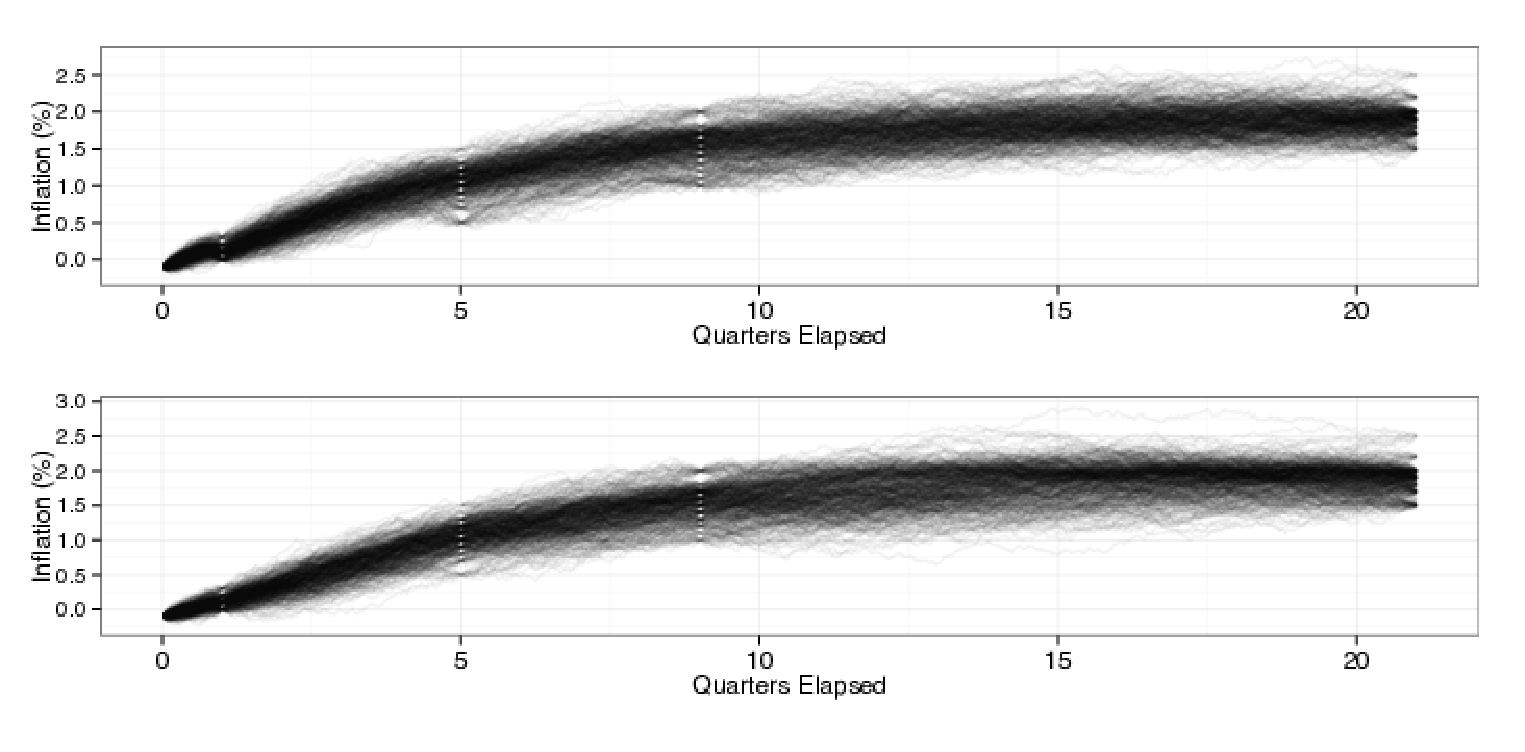
\includegraphics[width=1\columnwidth]{/Users/marshall/Documents/senior/thesis/figures/cont_path}

\caption{\label{fig:cont_path}500 sample paths of $\hat{\nu}$-bridges of
$X$ under $\mathbb{Q}_{\theta^{*}}^{OU}$ (top) and $\mathbb{Q}_{\theta^{*}}^{HYP}$
(bottom), where $\theta^{*}$ is the MKLDE of $\mathbb{Q}_{\theta}^{OU}$
and $\mathbb{Q}_{\theta}^{HYP}$ from $\mathbb{P}$ respectively,
using the 2015Q4 SPF.}
\end{figure}


We conclude this chapter with a visualization of the final product
of this thesis in \figref{cont_path}. Using an approximate MCEM scheme
to infer the MKLDE of $\mathbb{Q}_{\theta}^{OU}$ and $\mathbb{Q}_{\theta}^{HYP}$
given $\hat{\nu}$, we plot repeated samples of $\hat{\nu}$-bridges
of $X$ under $\mathbb{Q}_{\theta^{*}}^{OU}$ and $\mathbb{Q}_{\theta^{*}}^{HYP}$
for the most recently conducted SPF (2015Q4). This figure highlights
the differences in behavior of the two diffusions when far from the
mean. In particular, the shortcomings of the time-homogenous OU model's
linear mean reversion are laid bare: the imputed paths revert to the
inflation target far too quickly initially before being forced down
to the relatively low inflation expectations at the end of the 2015.
Time-inhomogeneity therefore appears to be an important feature of
inflation expectations as of 2015Q4, with expected inflation remaining
low in the short-term, and rapidly accelerating in the medium-term.
However, this is a problem of model selection and not of methodology;
as such, \figref{cont_path}, representing the synthesis of the methods
developed here to perform inference and imputation on the forecasts
of modern-day macroeconomic oracles, is a fitting conclusion to the
original portion of this thesis.
